\begin{beginningnote}
    Si tenga presente che alcuni termini utilizzati nel documento riportano la lettera \textbf{G} in apice, allo scopo di evidenziare le parole che assumono uno specifico significato nell'ambito del progetto. Per comprenderle in maniera corretta, si rimanda il lettore al documento ``Glossario", che contiene un elenco completo di tutte le terminologie utilizzate con relative definizioni, allo scopo di costruire un linguaggio uniforme che possa migliorare la comunicazione tra i componenti interni al gruppo e gli stakeholders\textsuperscript{G} esterni.   %inserire corsivo per ogni termine del glossario?
\end{beginningnote}

%unire scopo delcoumento e il progetto in un unica sezione  (e.g. introduzione) con due sottosezioni?
%%%%%%%%%%%%%%%%%%%%%%%%%%%%%%%%%%%
% SCOPO DEL DOCUMENTO
%%%%%%%%%%%%%%%%%%%%%%%%%%%%%%%%%%%

\section{Introduzione}

\subsection{Scopo del documento}\label{sec:scopo_del_documento}
\par Questo documento definisce come le attività di controllo della qualità saranno gestite durante il ciclo di vita del prodotto software. Include dettagli sui processi e standard da seguire per assicurare che il prodotto finale rispetti i requisiti di qualità specificati. Questo piano è fondamentale per garantire che il software sviluppato sia di alta qualità e soddisfi le aspettative dei clienti e degli stakeholder. Al suo interno contiene le metriche per misurare il livello di qualità di progetto in fase di sviluppo, in modo da poter migliorare alcune procedure se giudicate non conformi alle aspettative. Si prevede che il documento abbia natura incrementale, perché le metriche potrebbero essere aggiornate o riadattate in corso di progetto, a seconda delle esigenze e delle richieste da parte del committente.
\par Nel corso di progetto, l'accertamento della qualità sarà documentato allegando al documento le misurazioni delle attività di verifica con le metriche descritte.

%%%%%%%%%%%%%%%%%%%%%%%%%%%%%%%%%%%
% IL PROGETTO
%%%%%%%%%%%%%%%%%%%%%%%%%%%%%%%%%%%
\subsection{Il progetto}\label{sec:il_progetto}
\par Il progetto nasce nell'ambito dei \textbf{sistemi gestionali di magazzino}, meglio noti con il termine inglese di \textit{Warehouse Management Systems} (WMS), con l'obiettivo di risolvere una serie di problematiche derivanti dalle soluzioni tradizionali tuttora presenti sul mercato.
\par Il focus principale sarà migliorare la user experience, tramite la realizzazione di un applicativo che proponga all'utente un'interazione con il magazzino in un ambiente di lavoro 3D: questa soluzione, rispetto ai tradizionali sistemi 2D, garantirebbe una maggiore comprensione degli spazi, proponendo una visualizzazione più intuitiva e familiare del magazzino all'utente che, di conseguenza, sarà in grado di prendere decisioni organizzative più informate ed efficienti, ottimizzando i processi di logistica.
\par Per raggiungere questo obiettivo, l'ambiente di lavoro non può essere una semplice visualizzazione del magazzino. L'utente dovrà infatti poter:
\begin{itemize}
    \item Navigare l'ambiente 3D;
    \item Progettare la scaffalatura e modificarla nel tempo;
    \item Inserire, spostare e rimuovere prodotti negli scaffali.
\end{itemize}
Il progetto deve concretizzarsi nella realizzazione di una web app fruibile agli impiegati d'ufficio ed incentrata sulla visualizzazione 3D del magazzino.
\par Per visionare il capitolato\textsuperscript{G} e la documentazione del gruppo, si veda la sezione \hyperref[sec:riferimenti_esterni]{Riferimenti Esterni} del documento.


\newpage

%%%%%%%%%%%%%%%%%%%%%%%%%%%%%%%%%%%
% METRICHE
%%%%%%%%%%%%%%%%%%%%%%%%%%%%%%%%%%%
\section{Metriche}\label{sec:metriche}
\subsection{Codice}
Le metriche descritte nel documento saranno identificate univocamente tramite un codice standardizzato dal gruppo nella seguente maniera:
\begin{center}
    \textbf{M[Tipo][Identificativo]-[Acronimo]}
\end{center}
dove:
\begin{itemize}
    \item \textbf{Tipo:} indica se la metrica misura la qualità di:
        \begin{itemize}
            \item \textbf{PC}: un processo;
            \item \textbf{PD}: un prodotto.
        \end{itemize}                 
    \item \textbf{Identificativo:} si tratta di un numero progressivo univoco all'interno di uno stesso \textit{Tipo}.
    \item \textbf{Acronimo:} indica l'acronimo del nome della metrica.
\end{itemize}
\subsection{Contenuto}
Per ogni metrica verranno riportati:
\begin{itemize}
    \item Una breve \textbf{descrizione};
    \item I \textbf{valori accettabili} in fase di controllo della qualità;
    \item I \textbf{valori ottimali} che la metrica dovrebbe raggiungere.
\end{itemize}


\newpage

%%%%%%%%%%%%%%%%%%%%%%%%%%%%%%%%%%%
% QUALITA' DI PROCESSO
%%%%%%%%%%%%%%%%%%%%%%%%%%%%%%%%%%%
\section{Qualità di processo}\label{sec:qualita_di_processo}
Questa sezione è dedicata alle metriche atte a misurare la qualità dei processi nel corso del progetto didattico, qui descritti seguendo lo standard \textbf{ISO/IEC 12207}, reperibile nella sezione \hyperref[sec:riferimenti_esterni]{Riferimenti Esterni} del documento.
\subsection{Processi primari}
\subsubsection{Fornitura}
Uno dei compiti principali del processo di fornitura è la gestione delle procedure e delle risorse necessarie a garantire il raggiungimento degli obiettivi di progetto. Per questo motivo, le metriche di qualità adottate in questo processo hanno lo scopo di misurare come il progetto si sta muovendo rispetto alla sua pianificazione originaria, in termini di costi previsti in partenza rispetto ai costi effettivi nel corso di progetto.
\par Risulta subito evidente il fatto che delle semplici metriche di monitoraggio dei tempi non sono abbastanza per comprendere lo stato effettivo del progetto (molte ore di lavoro non significano sempre che il prodotto da realizzare è a buon punto) e per questo non possono garantire un buon livello di qualità. Per questo motivo, il gruppo ha scelto di utilizzare le metriche proposte dal metodo \textbf{Earned Value}, che si propone di misurare la quantità di lavoro effettivamente eseguito su un progetto.
\par Gli acronimi utilizzati nelle metriche faranno riferimento a quelli proposti dallo standard, reperibili al link sulle metriche di progetto nella sezione \hyperref[sec:riferimenti_esterni]{Riferimenti Esterni}. Per una lettura più immediata del documento si riportano i termini principali:
\begin{table}[h!]
\centering
\def\arraystretch{1.5}
\begin{tabular}{ |m{2cm}|m{4cm}|m{8cm}| }
\hline
\rowcolor{lightgray!30}
\textbf{Acronimo} & \textbf{Nome} & \textbf{Significato}\\
\hline
\textbf{PV} & Planned Value & Costo pianificato per realizzare le attività di progetto alla data corrente.\\
\hline
\textbf{AC} & Actual Cost & Costo effettivamente sostenuto alla data corrente.\\
\hline
\textbf{EV} & Earned Value & Valore delle attività realizzate alla data corrente.\\
\hline
\textbf{BAC} & Budget at Completion & Indica il valore iniziale previsto per la realizzazione del progetto.\\
\hline
\textbf{ETC} & Estimate to Complete & Valore stimato per la realizzazione delle rimanenti attività necessarie al completamento del progetto.\\
\hline
\textbf{EAC} & Estimated at Completion & Indica la revisione del BAC rispetto allo stato corrente del progetto (EAC = AC + ETC).\\
\hline
\textbf{CV} & Cost Variance & Calcola il valore del costo realmente maturato rispetto al costo effettivo (CV = EV - AC).\\
\hline
\textbf{SV} & Schedule Variance & Calcola le tempistiche effettive (se si è in anticipo o ritardo) rispetto alla schedulazione delle attività pianificate (SV = EV - PV).\\
\hline
\textbf{BV} & Budget Variance & Indica se alla data corrente si è speso di più o di meno rispetto a quanto previsto (BV = PV - AC).\\
\hline
\end{tabular}
\end{table}

\newpage
Le metriche sono stabilite di conseguenza:
\begin{table}[h!]
\rowcolors{2}{lightgray!30}{white}
\centering
\def\arraystretch{1.5}
\begin{tabular}{ |>{\centering\arraybackslash}m{2.5cm}|>{\centering\arraybackslash}m{5.5cm}|>{\centering\arraybackslash}m{3cm}|>{\centering\arraybackslash}m{3cm}| }
\hline
\rowcolor{black}
\textbf{\color{white} Codice} & \textbf{\color{white} Descrizione} & \textbf{\color{white} Valore accettabile} & \textbf{\color{white} Valore ottimale}\\
\hline
MPC1-EAC & Si vuole che il costo attuale sia quanto più possibile in linea con quello pianificato originariamente & Errore massimo del $\pm 5$\% rispetto a BAC & = BAC \\
\hline
MPC2-CV & Si vuole che il valore delle attività completate (EV) sia corrispondente o maggiore del costo sostenuto (AC) & $\geq$ -10\% & $\geq$ 0 \\
\hline
MPC3-SV & Si vuole che il progetto produca con maggiore o uguale velocità rispetto a quanto pianificato & $\geq$ -10\% & $\geq$ 0 \\
\hline
MPC4-BV & Si vuole che i costi previsti nella pianificazione iniziale corrispondano a quelli effettivi & Errore massimo del $\pm 10$\% & 0 \\
\hline
MPC5-PV & I costi pianificati per le attività di progetto non devono sforare i costi originariamente pianificati & - & La somma dei costi di volta in volta deve essere $\leq$ BAC \\
\hline
MPC6-AC & I costi effettivi per le attività di progetto non devono sforare i costi pianificati nella revisione del BAC & - & La somma dei costi di volta in volta deve essere $\leq$ EAC \\
\hline
MPC7-EV & Il valore effettivo per le attività di progetto non deve sforare i costi pianificati nella revisione del BAC & - & La somma dei costi di volta in volta deve essere $\leq$ EAC \\
\hline
\end{tabular}
\end{table}

\subsubsection{Sviluppo}
Il processo di sviluppo definisce i compiti e le attività che il gruppo deve svolgere per la
realizzazione del prodotto software concorde con le esigenze del proponente ed, in particolare, si occupa delle attività di analisi dei requisiti, progettazione e codifica. Le metriche di qualità individuate per questo processo sono relative soprattutto alle ultime due attività.
\paragraph{Progettazione}
Per assicurare qualità nella fase di progettazione si è ritenuto importante utilizzare le metriche di \textbf{Structural fan-in} e \textbf{fan-out}, applicate a procedure e file con i seguenti acronimi:
\begin{table}[h!]
\centering
\def\arraystretch{1.5}
\begin{tabular}{ |m{2cm}|m{4cm}|m{8cm}| }
\hline
\rowcolor{lightgray!30}
\textbf{Acronimo} & \textbf{Nome} & \textbf{Significato}\\
\hline
\textbf{SFINp} & Structural fan-in (procedure) & Numero di procedure che chiamano una specifica procedura.\\
\hline
\textbf{SFOUTp} & Structural fan-out (procedure) & Numero di procedure che una specifica procedura chiama.\\
\hline
\textbf{SFINf} & Structural fan-in (file) & Numero di file che hanno bisogno di uno specifico file per funzionare.\\
\hline
\textbf{SFOUTf} & Structural fan-out (file) & Numero di file da cui dipende (di cui ha bisogno) uno specifico file. \\
\hline
\end{tabular}
\end{table}

\newpage
Le regole da applicare alle metriche sono dunque le seguenti:
\begin{table}[h!]
\rowcolors{2}{lightgray!30}{white}
\centering
\def\arraystretch{1.5}
\begin{tabular}{ |>{\centering\arraybackslash}m{4cm}|>{\centering\arraybackslash}m{5.5cm}|>{\centering\arraybackslash}m{5cm}| }
\hline
\rowcolor{black}
\textbf{\color{white} Codice} & \textbf{\color{white} Descrizione} & \textbf{\color{white} Valore desiderabile}\\
\hline
MPC8-SFINp & Si vuole che le procedure progettate vengano riutilizzate & Alto (riutilizzo di codice) \\
\hline
MPC9-SFOUTp & Si vuole che le procedure non siano fortemente accoppiate fra loro & Basso (bassa dipendenza tra procedure) \\
\hline
MPC10-SFINf & Il numero di file che utilizzano uno specifico file non deve essere troppo alto per evitare dipendenze tra file & Ragionevolmente basso (bassa dipendenza tra file) \\
\hline
MPC11-SFOUTf & Il livello di accoppiamento tra file deve essere basso & Basso (bassa dipendenza tra file) \\
\hline
\end{tabular}
\end{table}

\paragraph{Codifica}
Con l'attività di codifica, i programmatori si impegnano a concretizzare quanto prodotto con l'attività di progettazione attraverso la programmazione del software vero e proprio.
Lo scopo è quello di ottenere un prodotto software che rispetti i requisti e le richieste concordati con il proponente e che ne garantisca la qualità. Per raggiungere questi obiettivi si utilizzano metriche che cercano di limitare gli errori introdotti nel codice, in particolare:
\begin{table}[h!]
\centering
\def\arraystretch{1.5}
\begin{tabular}{ |m{2cm}|m{2.5cm}|m{9.5cm}| }
\hline
\rowcolor{lightgray!30}
\textbf{Acronimo} & \textbf{Nome} & \textbf{Significato}\\
\hline
\textbf{CCH} & Code churn & Indica il numero di modifiche, aggiunte e cancellazioni apportate nel tempo ad una certa area di codice, in particolare nell'ambito di progetto, si intende modifiche apportate ad una procedura. Più sono le modifiche, più aumenta il rischio di introdurre errori nel codice. Un alto valore di nuove linee di codice potrebbe anche indicare basso riutilizzo di codice.\\
\hline
\textbf{NB} & Number of bugs & Indica il numero di bug ed errori presenti nel software.\\
\hline
\textbf{CC} & Cyclomatic complexity & Misura la complessità del codice calcolando il numero di percorsi indipendenti (contando cioè il numero di ``decisioni prese" nel codice sorgente). Un alto valore di complessità ciclomatica\textsuperscript{G} indica codice difficile da comprendere, mantenere e testare.\\
\hline
\end{tabular}
\end{table}
\par Le regole di qualità sono applicate alle metriche nel seguente modo:
\begin{table}[h!]
\rowcolors{2}{lightgray!30}{white}
\centering
\def\arraystretch{1.5}
\begin{tabular}{ |>{\centering\arraybackslash}m{2.5cm}|>{\centering\arraybackslash}m{5.5cm}|>{\centering\arraybackslash}m{3cm}|>{\centering\arraybackslash}m{3cm}| }
\hline
\rowcolor{black}
\textbf{\color{white} Codice} & \textbf{\color{white} Descrizione} & \textbf{\color{white} Valore accettabile} & \textbf{\color{white} Valore ottimale}\\
\hline
MPC12-CCH & Il numero di modifiche apportate alla singola procedura deve essere quanto più basso possibile & massimo 20\% di modifiche sul codice totale della procedura & 0 \\
\hline
MPC13-NB & Si vuole che il numero di bug ed errori nel codice sia quanto più basso possibile & $\leq$ 5 & 0 \\
\hline
MPC14-CC & Il codice deve essere mantenuto semplice, facilitando comprensione, manutenzione e test & $\leq$ 15 & $\leq$ 10 \\
\hline
\end{tabular}
\end{table}

\subsection{Processi di supporto}
\subsubsection{Documentazione}
La documentazione prodotta nel corso del progetto deve essere un valido supporto al gruppo e agli stakeholders per comprendere meglio il codice prodotto, le decisioni prese e la gestione organizzativa. Per questo motivo, le metriche di qualità sulla documentazione si concentrano sulla leggibilità e sul controllo degli errori ortografici. Le metriche in questione sono le seguenti:
\begin{table}[h!]
\centering
\def\arraystretch{1.5}
\begin{tabular}{ |m{2cm}|m{4.5cm}|m{7.5cm}| }
\hline
\rowcolor{lightgray!30}
\textbf{Acronimo} & \textbf{Nome} & \textbf{Significato}\\
\hline
\textbf{EOD} & Errori ortografici per documento & Indica il numero di errori ortografici individuati per documento.\\
\hline
\textbf{IG} & Indice Gulpease & Calcola la leggibilità di un testo in lingua italiana prendendo in considerazione la lunghezza della parola e la lunghezza della frase rispetto al numero di lettere. 
\begin{center}
    $89 + \ddfrac{300 * (num.\: frasi) - 10 * (num.\: lettere)}{(num.\: parole)} $
\end{center}\\
\hline
\end{tabular}
\end{table}
\par Le regole di qualità sono applicate alle metriche nel seguente modo:
\begin{table}[h!]
\rowcolors{2}{lightgray!30}{white}
\centering
\def\arraystretch{1.5}
\begin{tabular}{ |>{\centering\arraybackslash}m{2.5cm}|>{\centering\arraybackslash}m{5.5cm}|>{\centering\arraybackslash}m{3cm}|>{\centering\arraybackslash}m{3cm}| }
\hline
\rowcolor{black}
\textbf{\color{white} Codice} & \textbf{\color{white} Descrizione} & \textbf{\color{white} Valore accettabile} & \textbf{\color{white} Valore ottimale}\\
\hline
MPC15-EOD & Si vogliono meno errori ortografici possibili per ciascun documento & $\leq 5$ & 0 \\
\hline
MPC16-IG & La documentazione deve essere di facile lettura & 30-100 & 40-100 \\
\hline
\end{tabular}
\end{table}

\subsubsection{Accertamento della qualità}
Lo scopo dell'accertamento della qualità è garantire che i processi e il prodotto siano conformi alle attese e soddisfino al meglio le richieste del proponente. A tal fine e per avere una valutazione oggettiva e quantificabile della qualità, si fa riferimento al presente ``Piano di Qualifica", che riporta le metriche di qualità adottate dal gruppo nell'ambito del progetto.
\par Diventa quindi essenziale il soddisfacimento delle metriche preposte:
\begin{table}[h!]
\centering
\def\arraystretch{1.5}
\begin{tabular}{ |m{2cm}|m{3.5cm}|m{8.5cm}| }
\hline
\rowcolor{lightgray!30}
\textbf{Acronimo} & \textbf{Nome} & \textbf{Significato}\\
\hline
\textbf{MS} & Metriche soddisfatte & Indica la percentuale di metriche di qualità soddisfatte rispetto al totale delle metriche preposte.\\
\hline
\end{tabular}
\end{table}
\par Con le seguenti regole:
\begin{table}[h!]
\rowcolors{2}{lightgray!30}{white}
\centering
\def\arraystretch{1.5}
\begin{tabular}{ |>{\centering\arraybackslash}m{2.5cm}|>{\centering\arraybackslash}m{5.5cm}|>{\centering\arraybackslash}m{3cm}|>{\centering\arraybackslash}m{3cm}| }
\hline
\rowcolor{black}
\textbf{\color{white} Codice} & \textbf{\color{white} Descrizione} & \textbf{\color{white} Valore accettabile} & \textbf{\color{white} Valore ottimale}\\
\hline
MPC17-MS & Il numero di metriche di qualità soddisfatte deve essere molto alto & 90\% & 100\% \\
\hline
\end{tabular}
\end{table}

\newpage
\subsubsection{Verifica}
Il processo di verifica ha lo scopo di determinare se i prodotti dei processi durante il corso del progetto rispettano i requisiti preposti. In particolare, si vuole enfatizzare la correttezza del codice prodotto attraverso le seguenti metriche:
\begin{table}[h!]
\centering
\def\arraystretch{1.5}
\begin{tabular}{ |m{2cm}|m{3.5cm}|m{8.5cm}| }
\hline
\rowcolor{lightgray!30}
\textbf{Acronimo} & \textbf{Nome} & \textbf{Significato}\\
\hline
\textbf{CCV} & Code coverage & Misura la quantità di codice (in percentuale) coperta dai test rispetto al totale del codice sorgente.\\
\hline
\textbf{TP} & Test passati & Misura la quantità di test (in percentuale) eseguiti con successo.\\
\hline
\end{tabular}
\end{table}
\par Con le seguenti regole:
\begin{table}[h!]
\rowcolors{2}{lightgray!30}{white}
\centering
\def\arraystretch{1.5}
\begin{tabular}{ |>{\centering\arraybackslash}m{2.5cm}|>{\centering\arraybackslash}m{5.5cm}|>{\centering\arraybackslash}m{3cm}|>{\centering\arraybackslash}m{3cm}| }
\hline
\rowcolor{black}
\textbf{\color{white} Codice} & \textbf{\color{white} Descrizione} & \textbf{\color{white} Valore accettabile} & \textbf{\color{white} Valore ottimale}\\
\hline
MPC18-CCV & Si vuole che la percentuale di codice coperta da test sia molto alta & $\geq$ 90\% & 100\% \\
\hline
MPC19-TP & Si vuole che tutti i test siano eseguiti con successo & 100\% & 100\% \\
\hline
\end{tabular}
\end{table}
\newpage

\section{Qualità di prodotto}
L'obiettivo delle metriche definite in questa sezione è controllare la qualità del prodotto realizzato nel corso del progetto. Per questa ragione, diventa importante assicurarsi che il prodotto sia conforme alle richieste del proponente e che possieda le caratteristiche proprie di un software di qualità.
\subsection{Customer needs}
Si definiscono le seguenti metriche:
\begin{table}[h!]
\centering
\def\arraystretch{1.5}
\begin{tabular}{ |m{2cm}|m{5.5cm}|m{6.5cm}| }
\hline
\rowcolor{lightgray!30}
\textbf{Acronimo} & \textbf{Nome} & \textbf{Significato}\\
\hline
\textbf{ROB} & Copertura dei requisiti obbligatori & Indica il valore (in percentuale) di requisiti obbligatori che il prodotto soddisfa.\\
\hline
\textbf{RDE} & Copertura dei requisiti desiderabili & Indica il valore (in percentuale) di requisiti desiderabili che il prodotto soddisfa.\\
\hline
\end{tabular}
\end{table}
\par Con le seguenti regole:
\begin{table}[h!]
\rowcolors{2}{lightgray!30}{white}
\centering
\def\arraystretch{1.5}
\begin{tabular}{ |>{\centering\arraybackslash}m{2.5cm}|>{\centering\arraybackslash}m{5.5cm}|>{\centering\arraybackslash}m{3cm}|>{\centering\arraybackslash}m{3cm}| }
\hline
\rowcolor{black}
\textbf{\color{white} Codice} & \textbf{\color{white} Descrizione} & \textbf{\color{white} Valore accettabile} & \textbf{\color{white} Valore ottimale}\\
\hline
MPD1-ROB & I requisiti obbligatori devono essere tutti soddisfatti & 100\% & 100\% \\
\hline
MPD2-RDE & I requisiti desiderabili devono essere soddisfatti in buona parte & 70\% & 100\% \\
\hline
\end{tabular}
\end{table}

\subsection{Efficienza}
Si definiscono le seguenti metriche:
\begin{table}[h!]
\centering
\def\arraystretch{1.5}
\begin{tabular}{ |m{2cm}|m{5.5cm}|m{6.5cm}| }
\hline
\rowcolor{lightgray!30}
\textbf{Acronimo} & \textbf{Nome} & \textbf{Significato}\\
\hline
\textbf{ART} & Average response time & Misura il tempo medio che il prodotto software impiega per rispondere agli input forniti dall'utente.\\
\hline
\end{tabular}
\end{table}
\par Con le seguenti regole:
\begin{table}[h!]
\rowcolors{2}{lightgray!30}{white}
\centering
\def\arraystretch{1.5}
\begin{tabular}{ |>{\centering\arraybackslash}m{2.5cm}|>{\centering\arraybackslash}m{5.5cm}|>{\centering\arraybackslash}m{3cm}|>{\centering\arraybackslash}m{3cm}| }
\hline
\rowcolor{black}
\textbf{\color{white} Codice} & \textbf{\color{white} Descrizione} & \textbf{\color{white} Valore accettabile} & \textbf{\color{white} Valore ottimale}\\
\hline
MPD3-ART & Il prodotto deve essere veloce nel tempo di risposta & $<$ 3 sec. & $\leq$ 1 sec. \\
\hline
\end{tabular}
\end{table}

\subsection{Usabilità}
\par Si definiscono le seguenti metriche:
\begin{table}[h!]
\centering
\def\arraystretch{1.5}
\begin{tabular}{ |m{2cm}|m{5.5cm}|m{6.5cm}| }
\hline
\rowcolor{lightgray!30}
\textbf{Acronimo} & \textbf{Nome} & \textbf{Significato}\\
\hline
\textbf{PC} & Profondità di click per operazione & Misura il numero di click che l'utente deve fare per raggiungere un determinato obiettivo. Un numero troppo alto provoca frustrazione e difficoltà di utilizzo.\\
\hline
\textbf{CFO} & Comprensibilità funzioni offerte & Misura la quantità (in percentuale) di funzioni offerte che l'utente riesce ad individuare ed utilizzare con facilità.\\
\hline
\end{tabular}
\end{table}
\newpage
\par Con le seguenti regole:
\begin{table}[h!]
\rowcolors{2}{lightgray!30}{white}
\centering
\def\arraystretch{1.5}
\begin{tabular}{ |>{\centering\arraybackslash}m{2.5cm}|>{\centering\arraybackslash}m{5.5cm}|>{\centering\arraybackslash}m{3cm}|>{\centering\arraybackslash}m{3cm}| }
\hline
\rowcolor{black}
\textbf{\color{white} Codice} & \textbf{\color{white} Descrizione} & \textbf{\color{white} Valore accettabile} & \textbf{\color{white} Valore ottimale}\\
\hline
MPD4-PC & L'utente deve essere facilitato nell'interazione con il prodotto software & $\leq$ 7 & $\leq$ 5 \\
\hline
MPD5-CFO & L'utente deve comprendere facilmente quali sono e come si comportano le funzioni offerte & $\geq$ 90\% & 100\% \\
\hline
\end{tabular}
\end{table}

\subsection{Portabilità su altre piattaforme}
Su richiesta del committente, il software prodotto deve essere una Web Application. Come tale, risulta essenziale assicurarsi che il prodotto sia utilizzabile tramite tutti i browser maggiormente utilizzati nel mercato.
\par Le applicazioni che sono state considerate sono:
\begin{itemize}
    \item Google Chrome,
    \item Mozilla Firefox,
    \item Microsoft Edge,
    \item Safari,
    \item Opera.
\end{itemize}
Si definiscono dunque le seguenti metriche:
\begin{table}[h!]
\centering
\def\arraystretch{1.5}
\begin{tabular}{ |m{2cm}|m{5.5cm}|m{6.5cm}| }
\hline
\rowcolor{lightgray!30}
\textbf{Acronimo} & \textbf{Nome} & \textbf{Significato}\\
\hline
\textbf{PPT} & Portabilità su piattaforme & Indica la percentuale di piattaforme (tra quelle prese in considerazione) su cui il prodotto software è utilizzabile.\\
\hline
\end{tabular}
\end{table}
\par Con le seguenti regole:
\begin{table}[h!]
\rowcolors{2}{lightgray!30}{white}
\centering
\def\arraystretch{1.5}
\begin{tabular}{ |>{\centering\arraybackslash}m{2.5cm}|>{\centering\arraybackslash}m{5.5cm}|>{\centering\arraybackslash}m{3cm}|>{\centering\arraybackslash}m{3cm}| }
\hline
\rowcolor{black}
\textbf{\color{white} Codice} & \textbf{\color{white} Descrizione} & \textbf{\color{white} Valore accettabile} & \textbf{\color{white} Valore ottimale}\\
\hline
MPD6-PPT & Il prodotto deve essere utilizzabile su tutti i browser principali. & 100\% & 100\% \\
\hline
\end{tabular}
\end{table}

\subsection{Manutenibilità}
Si definiscono le seguenti metriche:
\begin{table}[h!]
\centering
\def\arraystretch{1.5}
\begin{tabular}{ |m{2cm}|m{5.5cm}|m{6.5cm}| }
\hline
\rowcolor{lightgray!30}
\textbf{Acronimo} & \textbf{Nome} & \textbf{Significato}\\
\hline
\textbf{CD} & Codice duplicato & Misura la quantità (in percentuale) di codice duplicato.\\
\hline
\end{tabular}
\end{table}
\par Con le seguenti regole:
\begin{table}[h!]
\rowcolors{2}{lightgray!30}{white}
\centering
\def\arraystretch{1.5}
\begin{tabular}{ |>{\centering\arraybackslash}m{2.5cm}|>{\centering\arraybackslash}m{5.5cm}|>{\centering\arraybackslash}m{3cm}|>{\centering\arraybackslash}m{3cm}| }
\hline
\rowcolor{black}
\textbf{\color{white} Codice} & \textbf{\color{white} Descrizione} & \textbf{\color{white} Valore accettabile} & \textbf{\color{white} Valore ottimale}\\
\hline
MPD7-CD & La duplicazione del codice deve essere minimizzata & $\leq$ 3\% & 0\% \\
\hline
\end{tabular}
\end{table}

\newpage
\section{Test}
\par Questa sezione è dedicata alla descrizione dei vari tipi di test che verranno effettuati per assicurare la qualità e l'affidabilità del software.

\subsection{Test di Unità}
\par I test di unità sono di basso livello e mirano a testare le singole unità dell'applicativo software in isolamento. Il concetto di unità si fa corrispondere generalmente alle funzioni per la programmazione procedurale, oppure a metodi e classi per la programmazione ad oggetti.
\par Sono i più economici da implementare, possono essere scritti più velocemente rispetto agli altri e generalmente vengono eseguiti in maniera automatica (rendendo veloce anche la loro esecuzione e ripetizione). Inoltre, permettono di individuare un problema in maniera più immediata, evitando che si propaghi nel software.

\subsection{Test di Integrazione}
\par I test di integrazione si pongono ad un livello più alto dei test di unità e sono eseguiti per controllare le interazioni tra le diverse componenti del software. L'obiettivo è verificare il corretto funzionamento delle componenti quando vengono integrate fra loro ed identificare problemi nelle interfacce e nelle interazioni.
\par Di norma sono eseguiti dopo i test di unità per verificare che le componenti che funzionano singolarmente continuino a funzionare in maniera corretta anche quando comunicano fra loro.

\subsection{Test di Sistema}
\par Sono eseguiti dopo aver completato i test sulle singole unità e sulla loro integrazione, con l'obiettivo di verificare il comportamento complessivo del sistema. Si basano sulle funzionalità espresse nei requisiti concordati con il proponente, per assicurare che tutte le richieste siano soddisfatte.

\subsection{Test di Regressione}
\par Sono eseguiti sulle nuove versioni del prodotto software per assicurarsi che le funzionalità aggiunte non abbiano introdotto errori nelle funzionalità preesistenti e che la qualità non sia regredita. Prevedono la ripetizione di tutto il processo di testing sulla nuova versione dell'applicativo, comprendente test di unità, integrazione e sistema.
%\par Eseguiti dopo ogni cambiamento al software per garantire che le nuove modifiche non introducano errori nelle parti già testate.
\begin{comment}
    \subsection{Test di Usabilità}
\par Valutazione dell'esperienza dell'utente con l'interfaccia del software, per garantire intuitività e facilità di uso.

\subsection{Test di Prestazione}
\par Controlli sulle prestazioni del software sotto vari carichi di lavoro, valutando tempo di risposta e scalabilità.
\end{comment}

\subsection{Test di Accettazione}
Sono test eseguiti poco prima del rilascio del prodotto, dopo aver già testato il software attraverso test di unità, integrazione e sistema. Gli obiettivi principali sono verificare che il software rispetta i requisiti prestabiliti con il cliente ed assicurarsi che sia pronto per essere rilasciato. Per questi motivi, vengono eseguiti alla presenza del committente e su un ambiente che sia quanto più vicino possibile a quello in cui si troverà a lavorare l'utente finale.

\newpage
\section{Resoconto}\label{resconto}

\subsection{Processi primari} \label{sec:processi_primari}
Di seguito sono visualizzati i grafici relativi alle metriche dei processi primari:

\subsubsection{MPC1-EAC}
\begin{figure}[h]
    \centering
    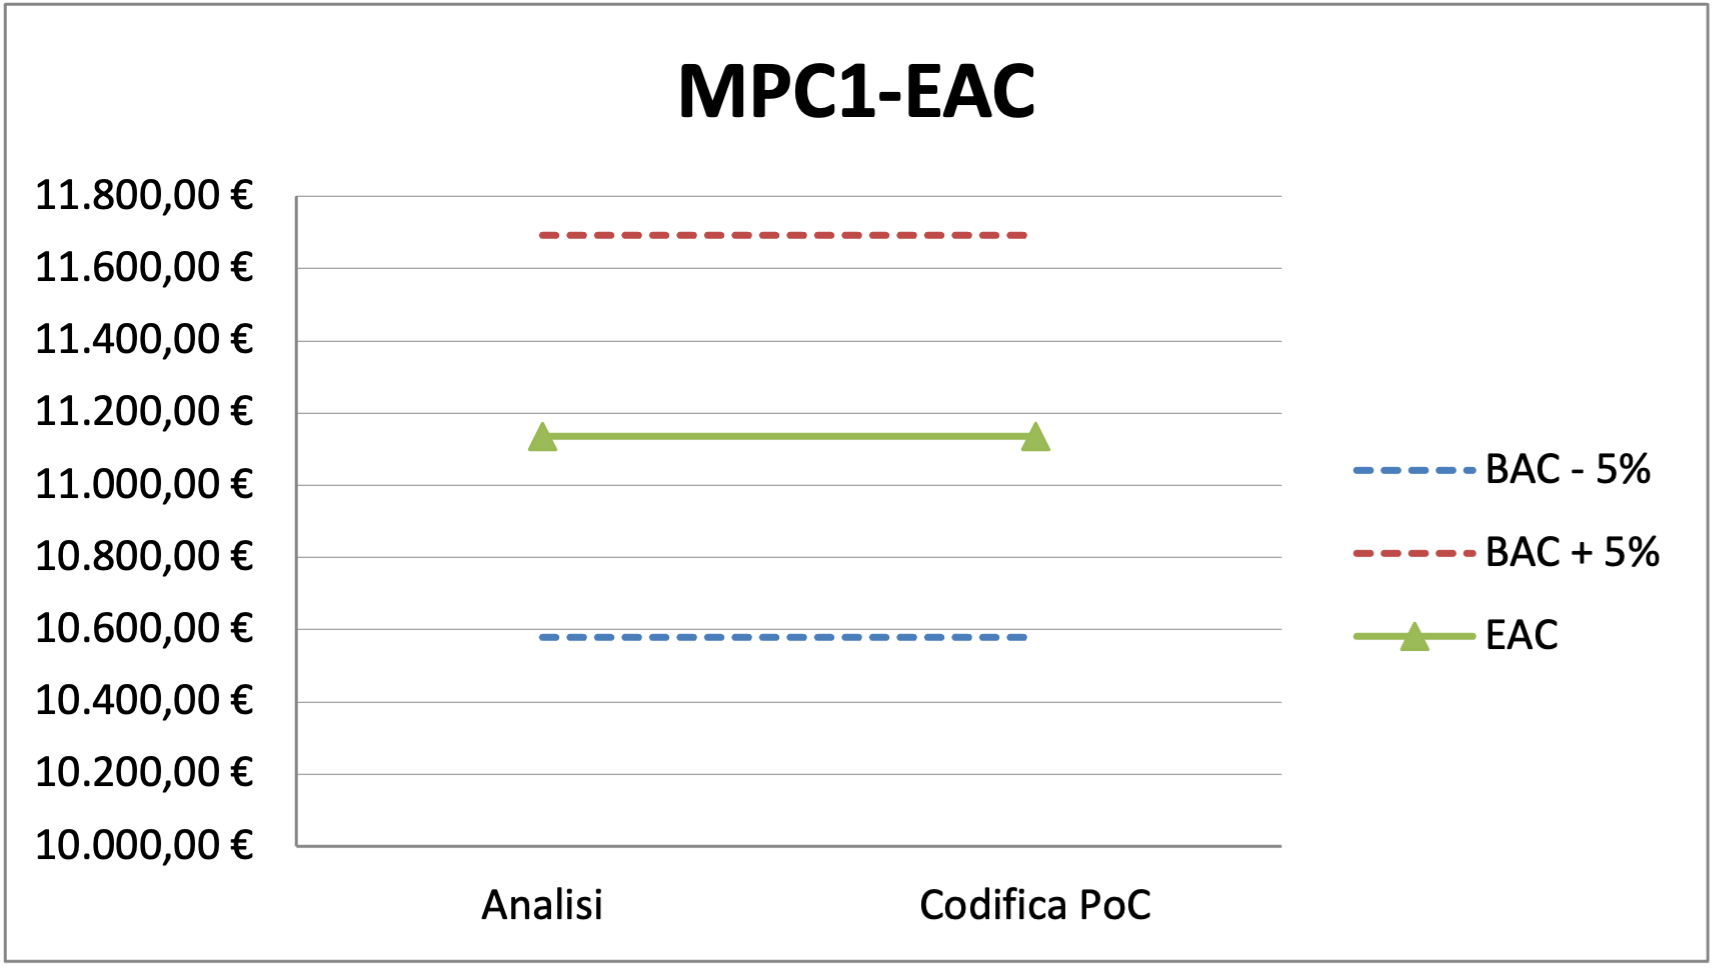
\includegraphics[width=0.8\textwidth]{images/MPC1-EAC.png}
    \caption{MPC1-EAC}
\end{figure}

\subsubsection{MPC2-CV}
\begin{figure}[h] 
    \centering
    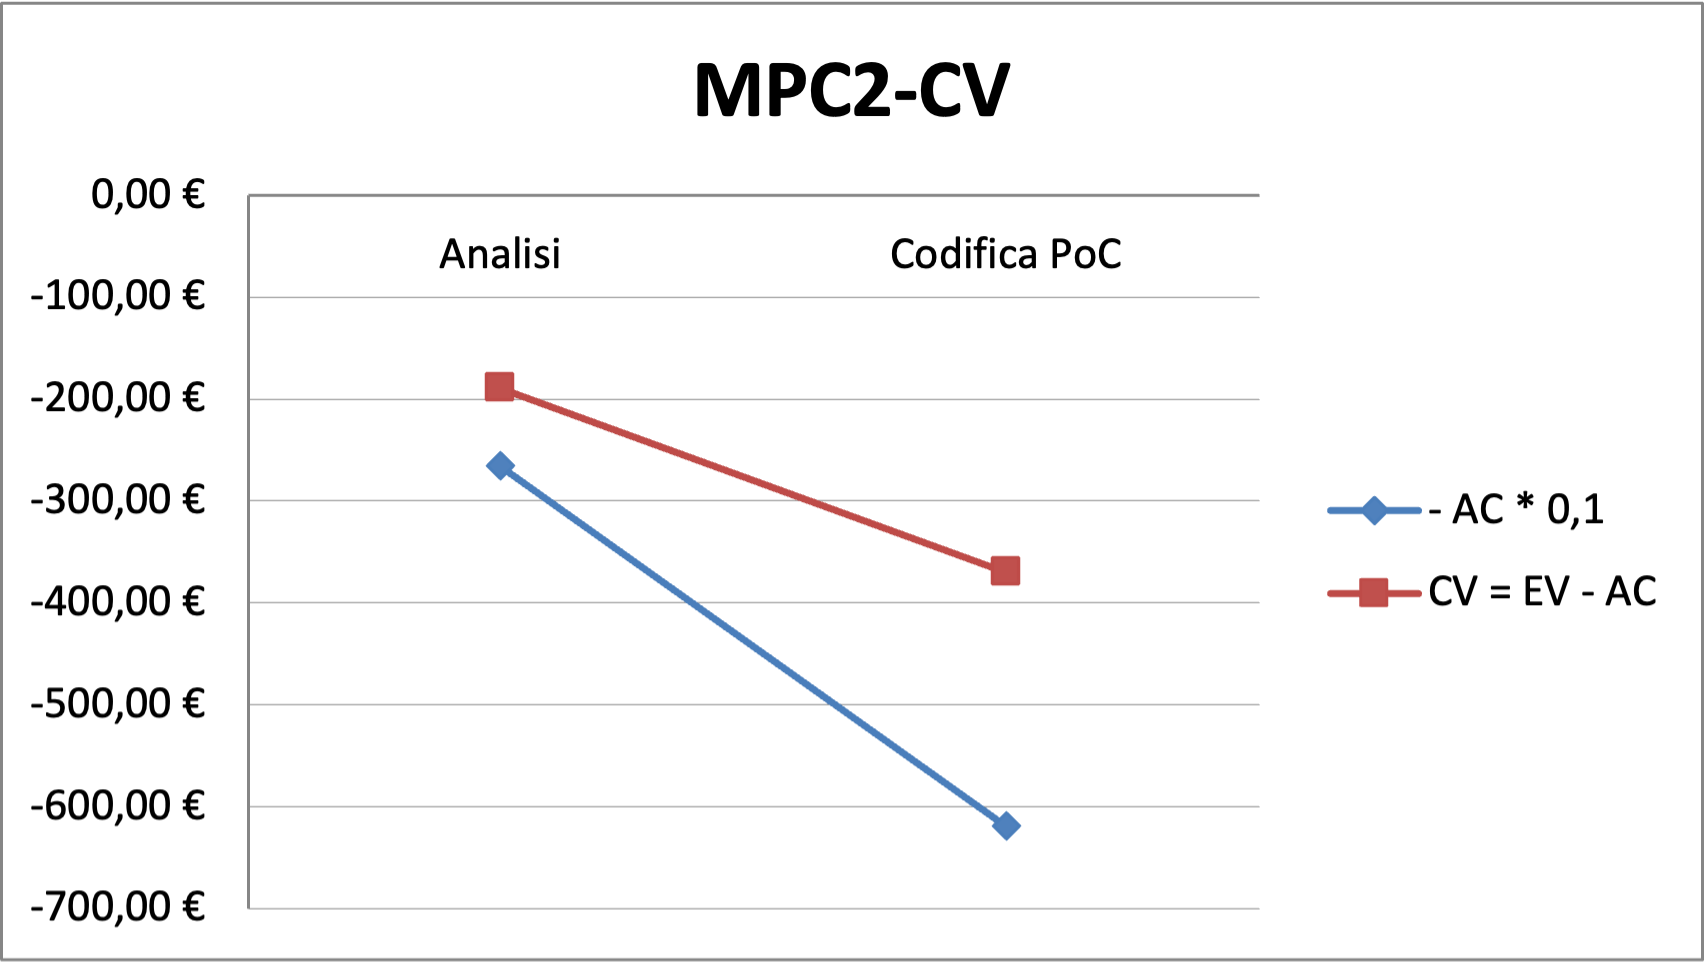
\includegraphics[width=0.8\textwidth]{images/MPC2-CV.png}
    \caption{MPC2-CV}
\end{figure}

\newpage

\subsubsection{MPC3-SV}
\begin{figure}[h]
    \centering
    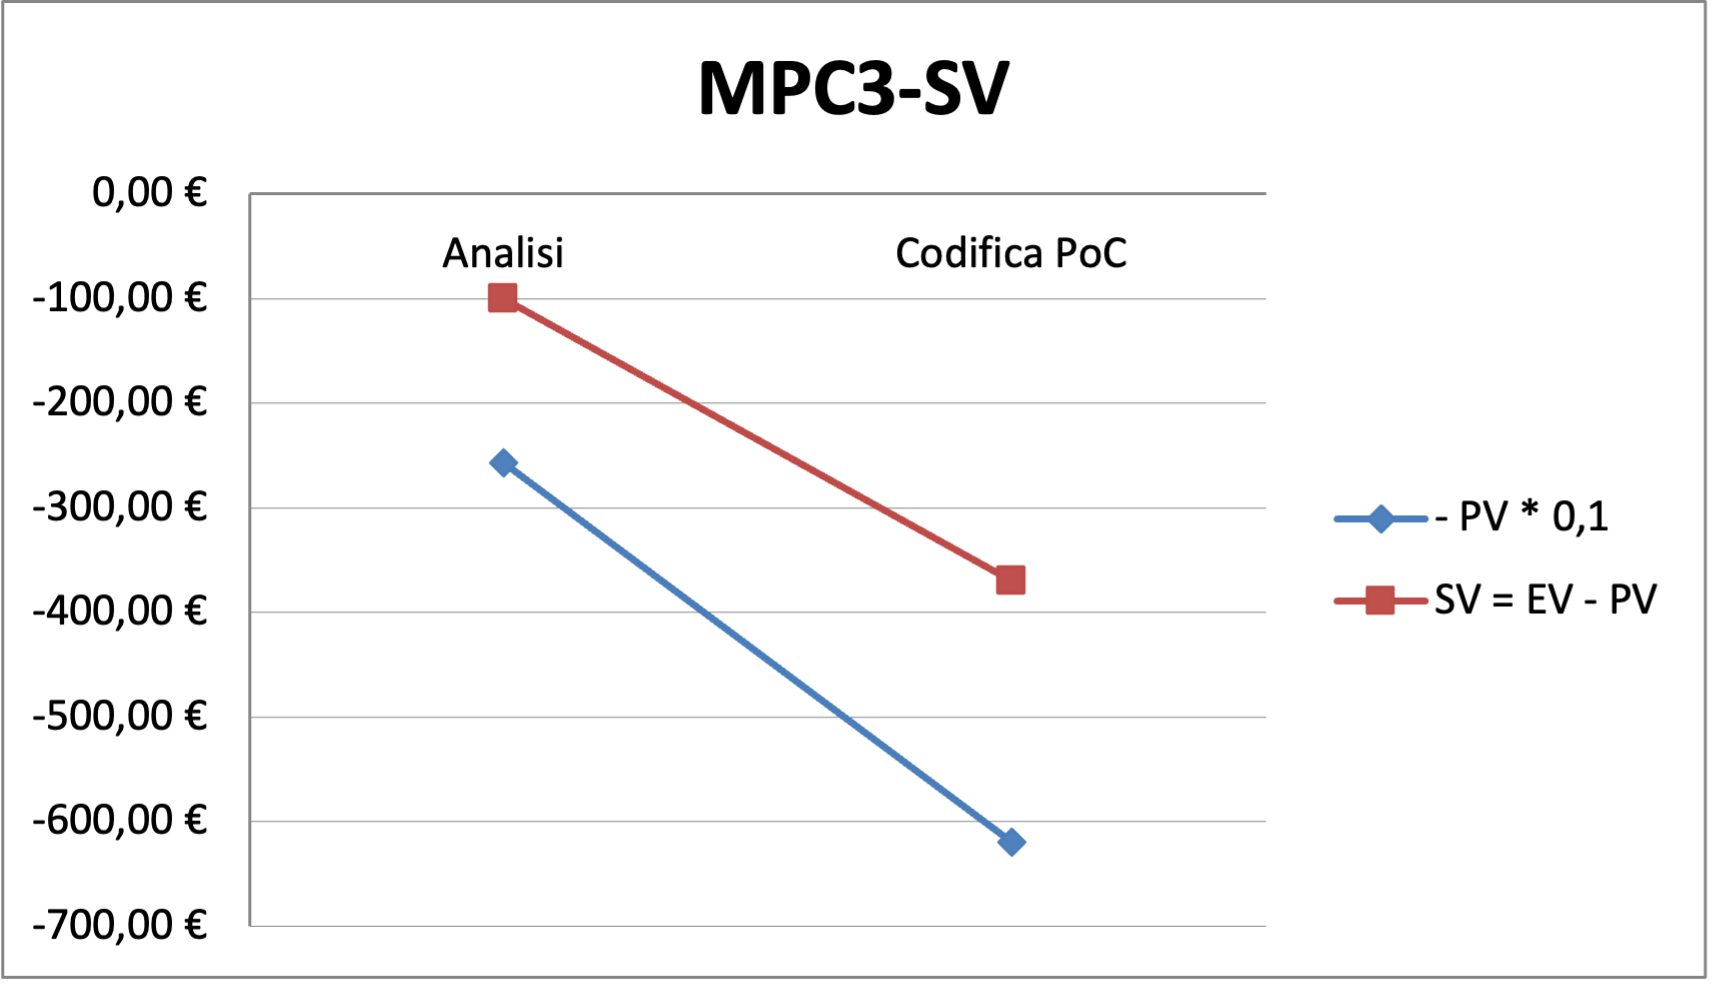
\includegraphics[width=0.8\textwidth]{images/MPC3-SV.png}
    \caption{MPC3-SV}
\end{figure}

\subsubsection{MPC4-BV}
\begin{figure}[h] 
    \centering
    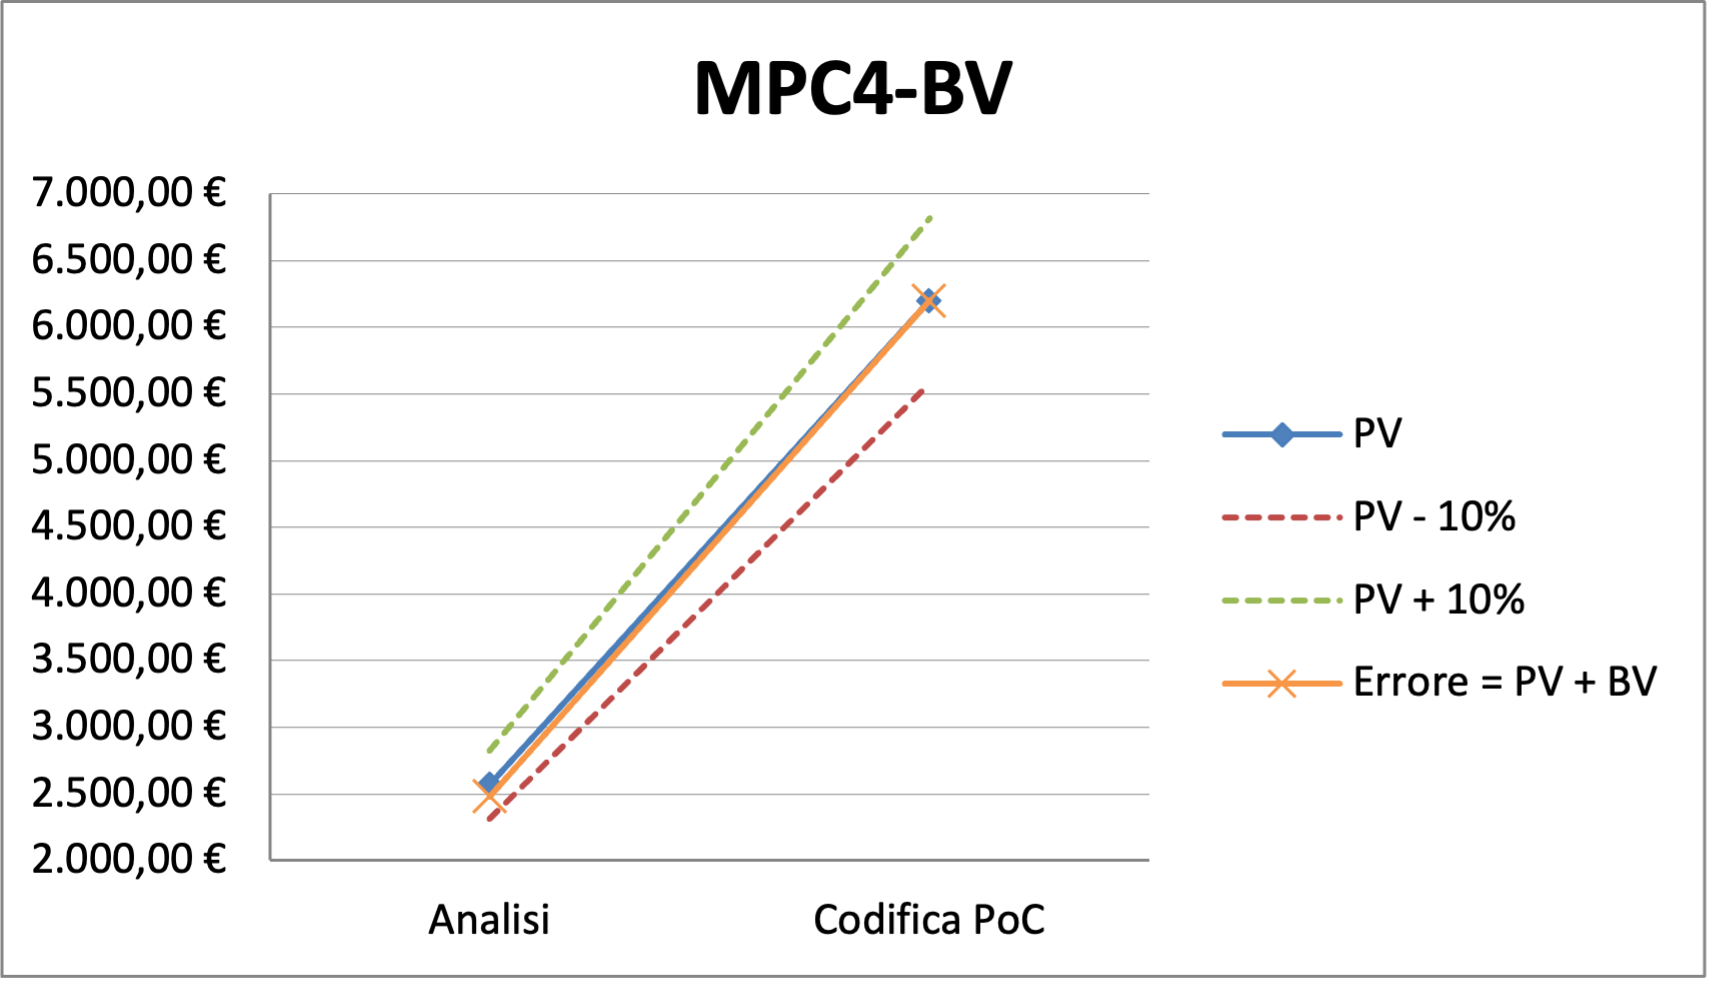
\includegraphics[width=0.8\textwidth]{images/MPC4-BV.png}
    \caption{MPC4-BV}
\end{figure}

\newpage

\subsubsection{MPC5-PV}
\begin{figure}[h]
    \centering
    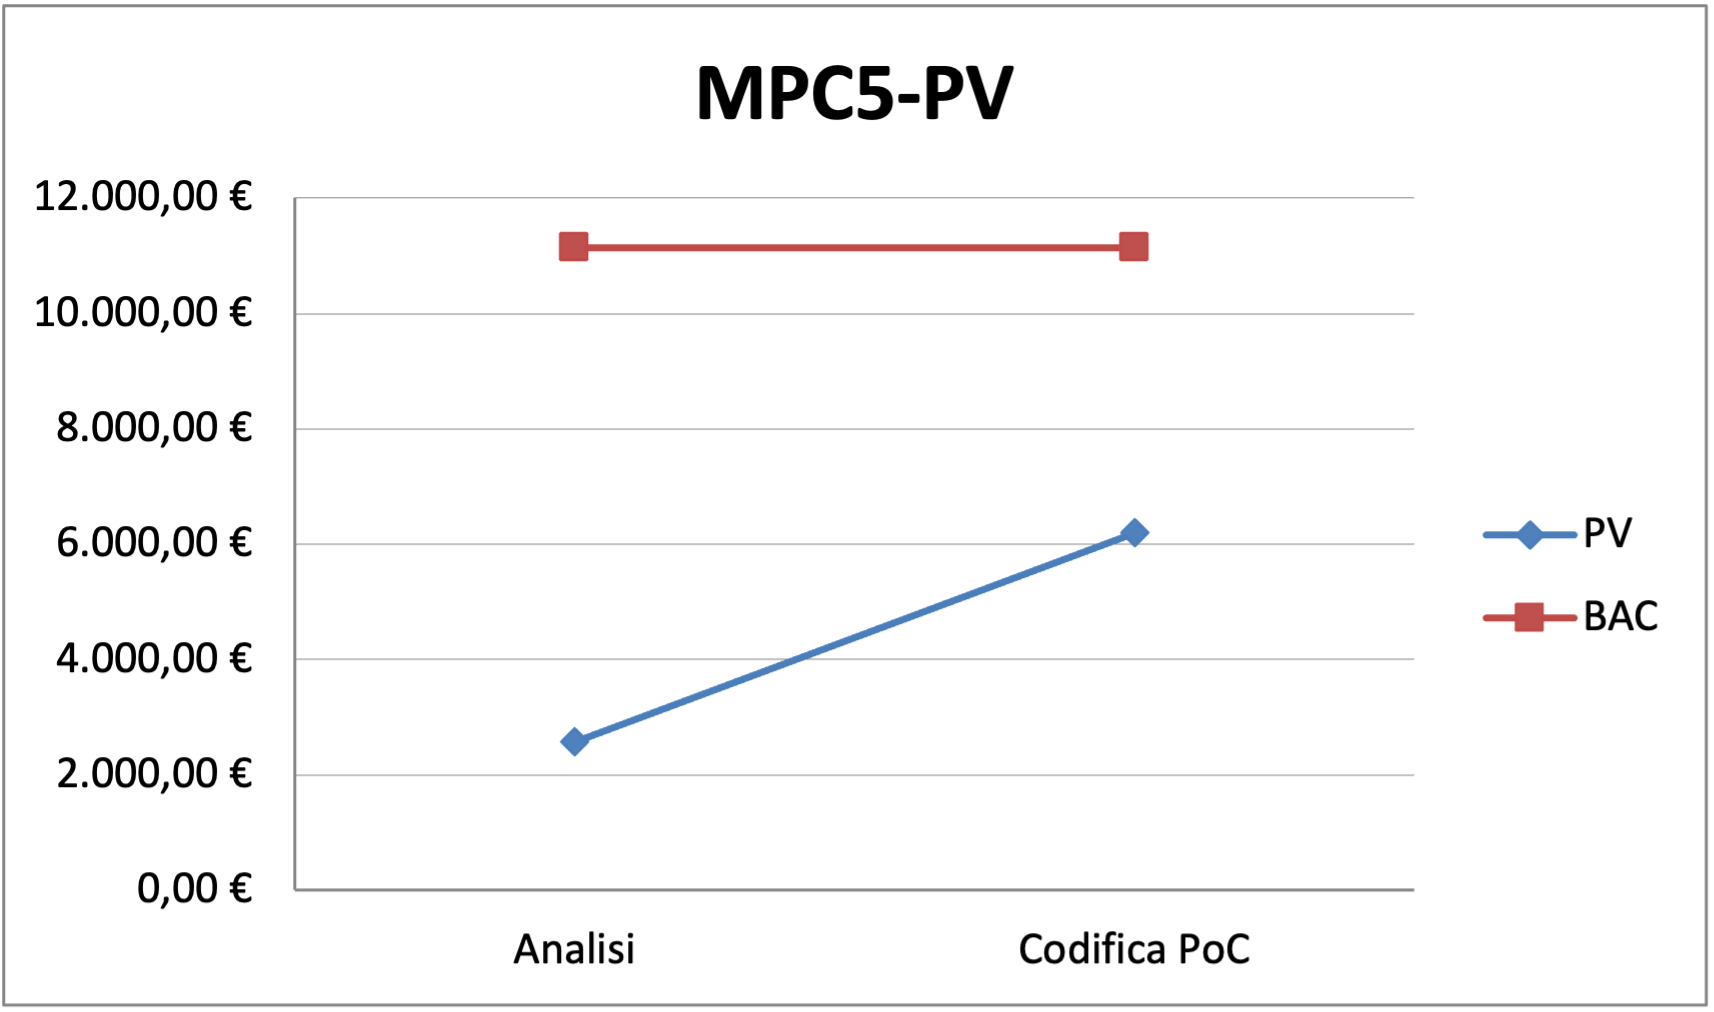
\includegraphics[width=0.8\textwidth]{images/MPC5-PV.png}
    \caption{MPC5-PV}
\end{figure}

\subsubsection{MPC6-AC}
\begin{figure}[h] 
    \centering
    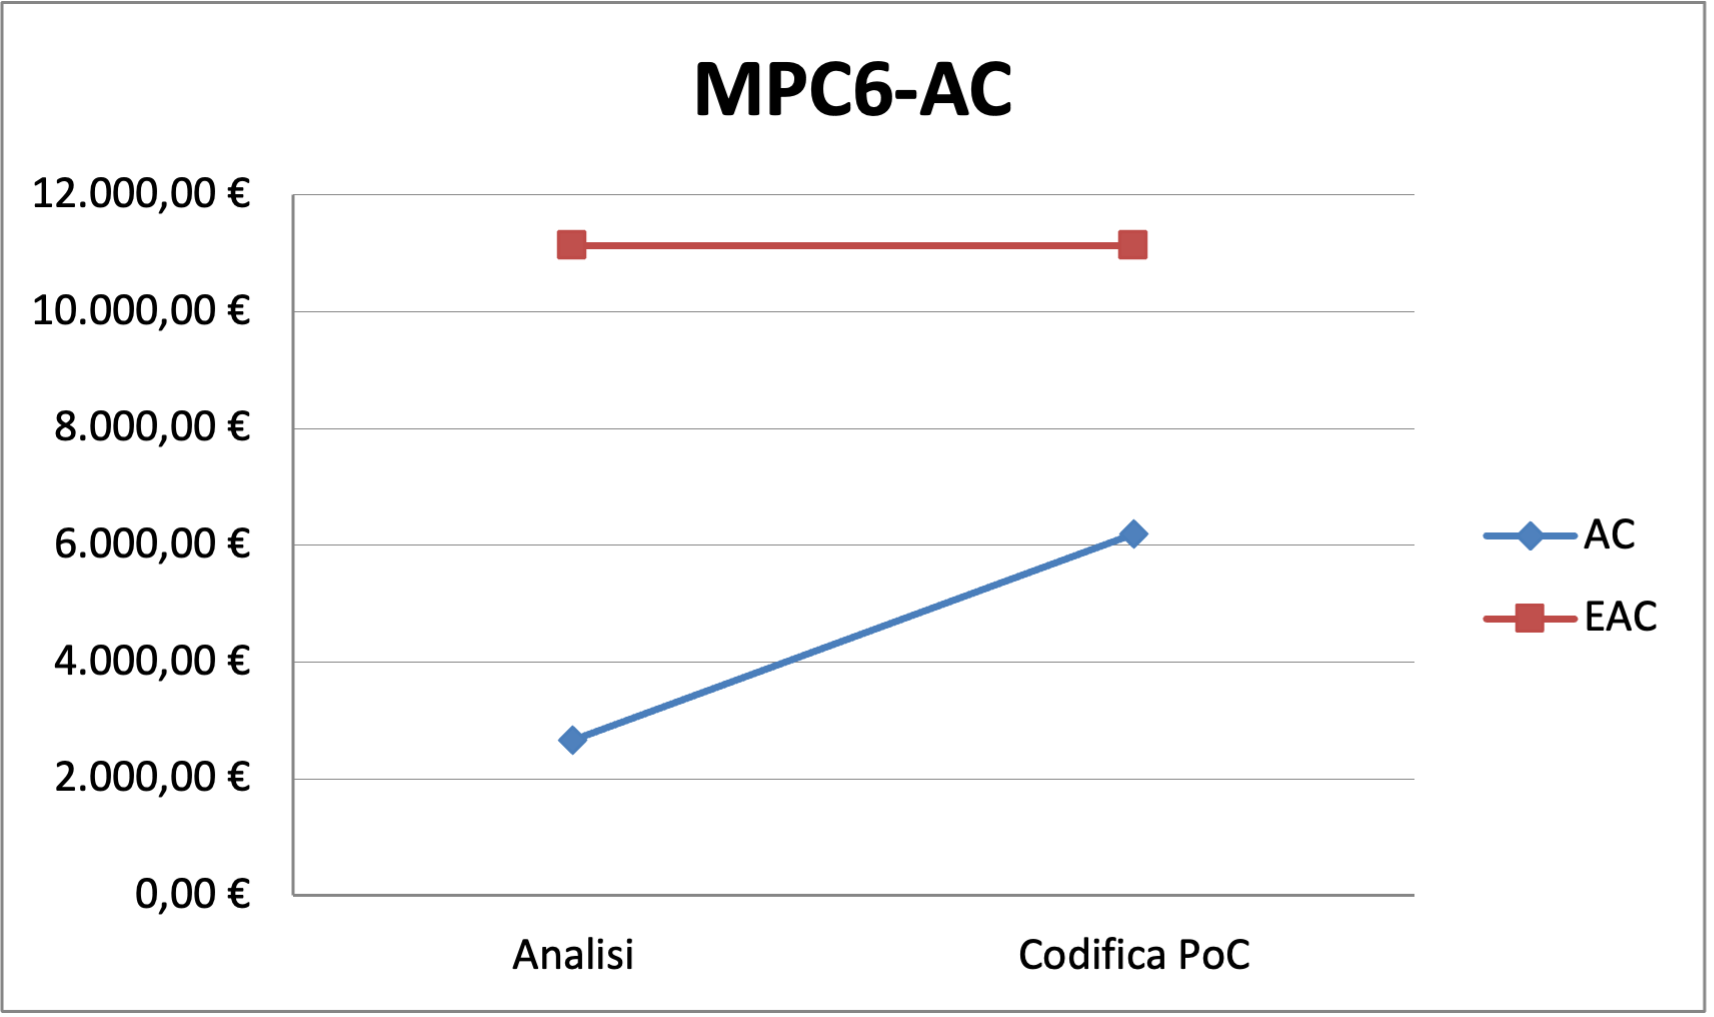
\includegraphics[width=0.8\textwidth]{images/MPC6-AC.png}
    \caption{MPC6-AC}
\end{figure}

\newpage

\subsubsection{MPC7-EV}
\begin{figure}[h] 
    \centering
    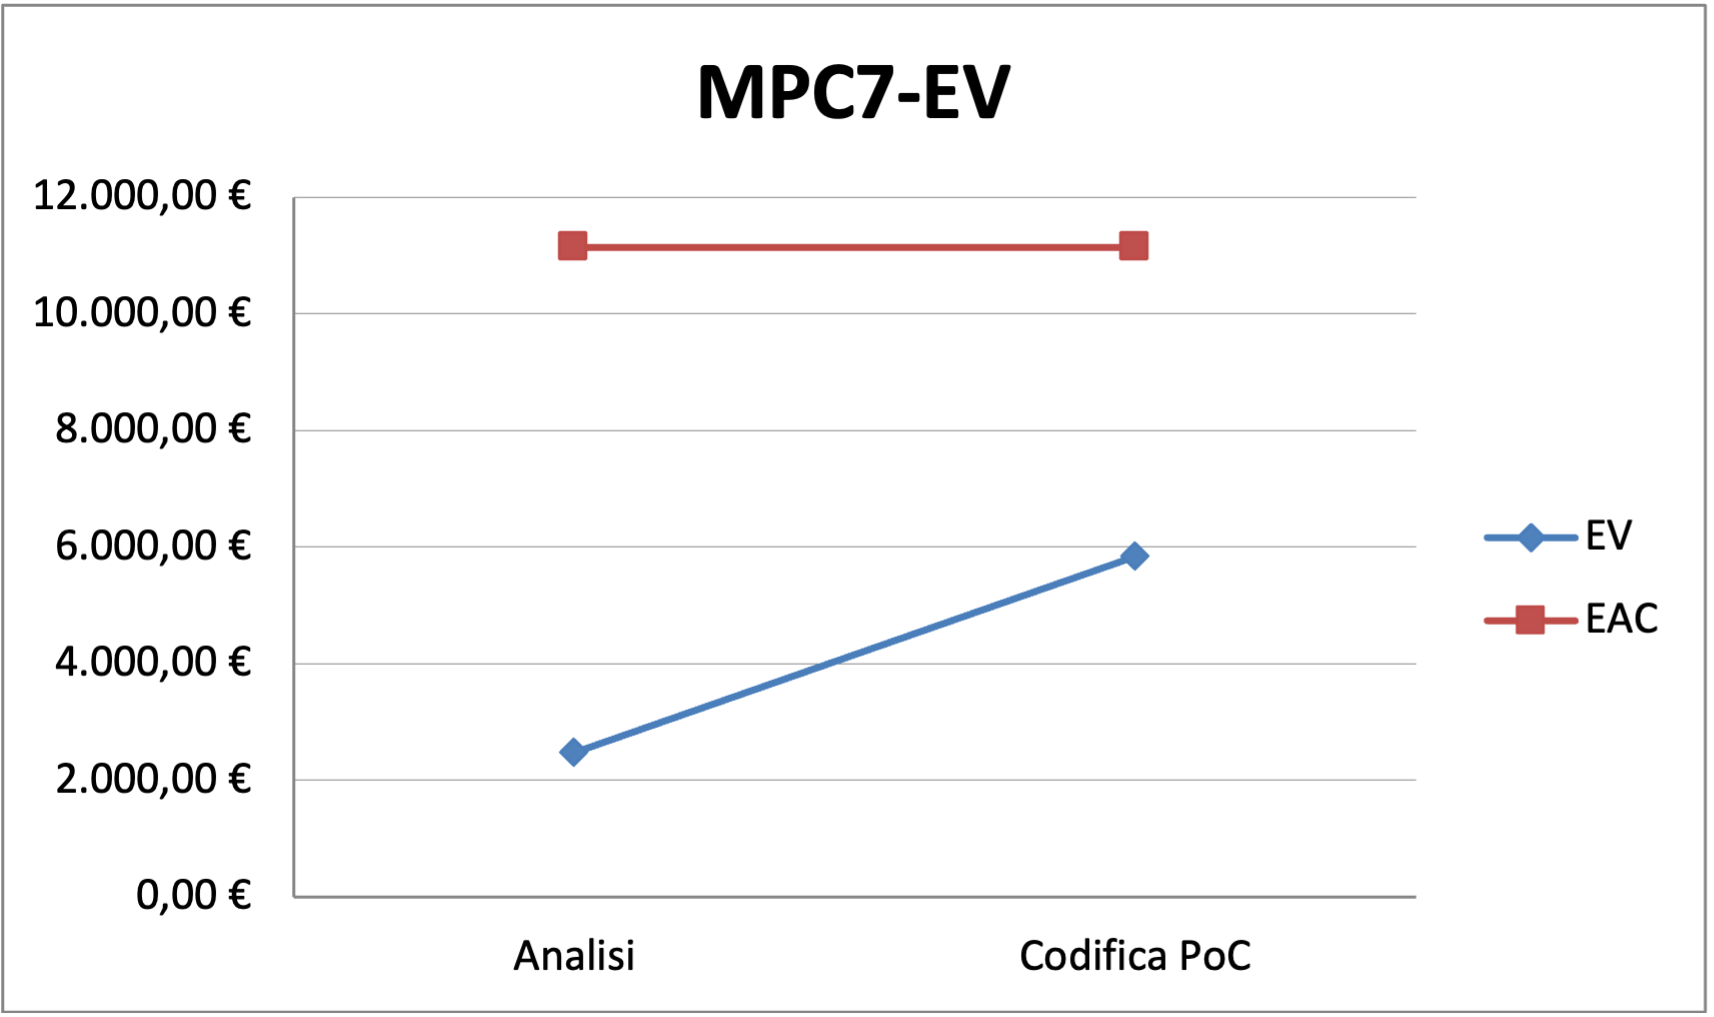
\includegraphics[width=0.8\textwidth]{images/MPC7-EV.png}
    \caption{MPC7-EV}
\end{figure}

\subsection{Processi di supporto} \label{sec:processi_di_supporto}

\subsubsection{MPC15-EOD}
\begin{figure}[h] 
    \centering
    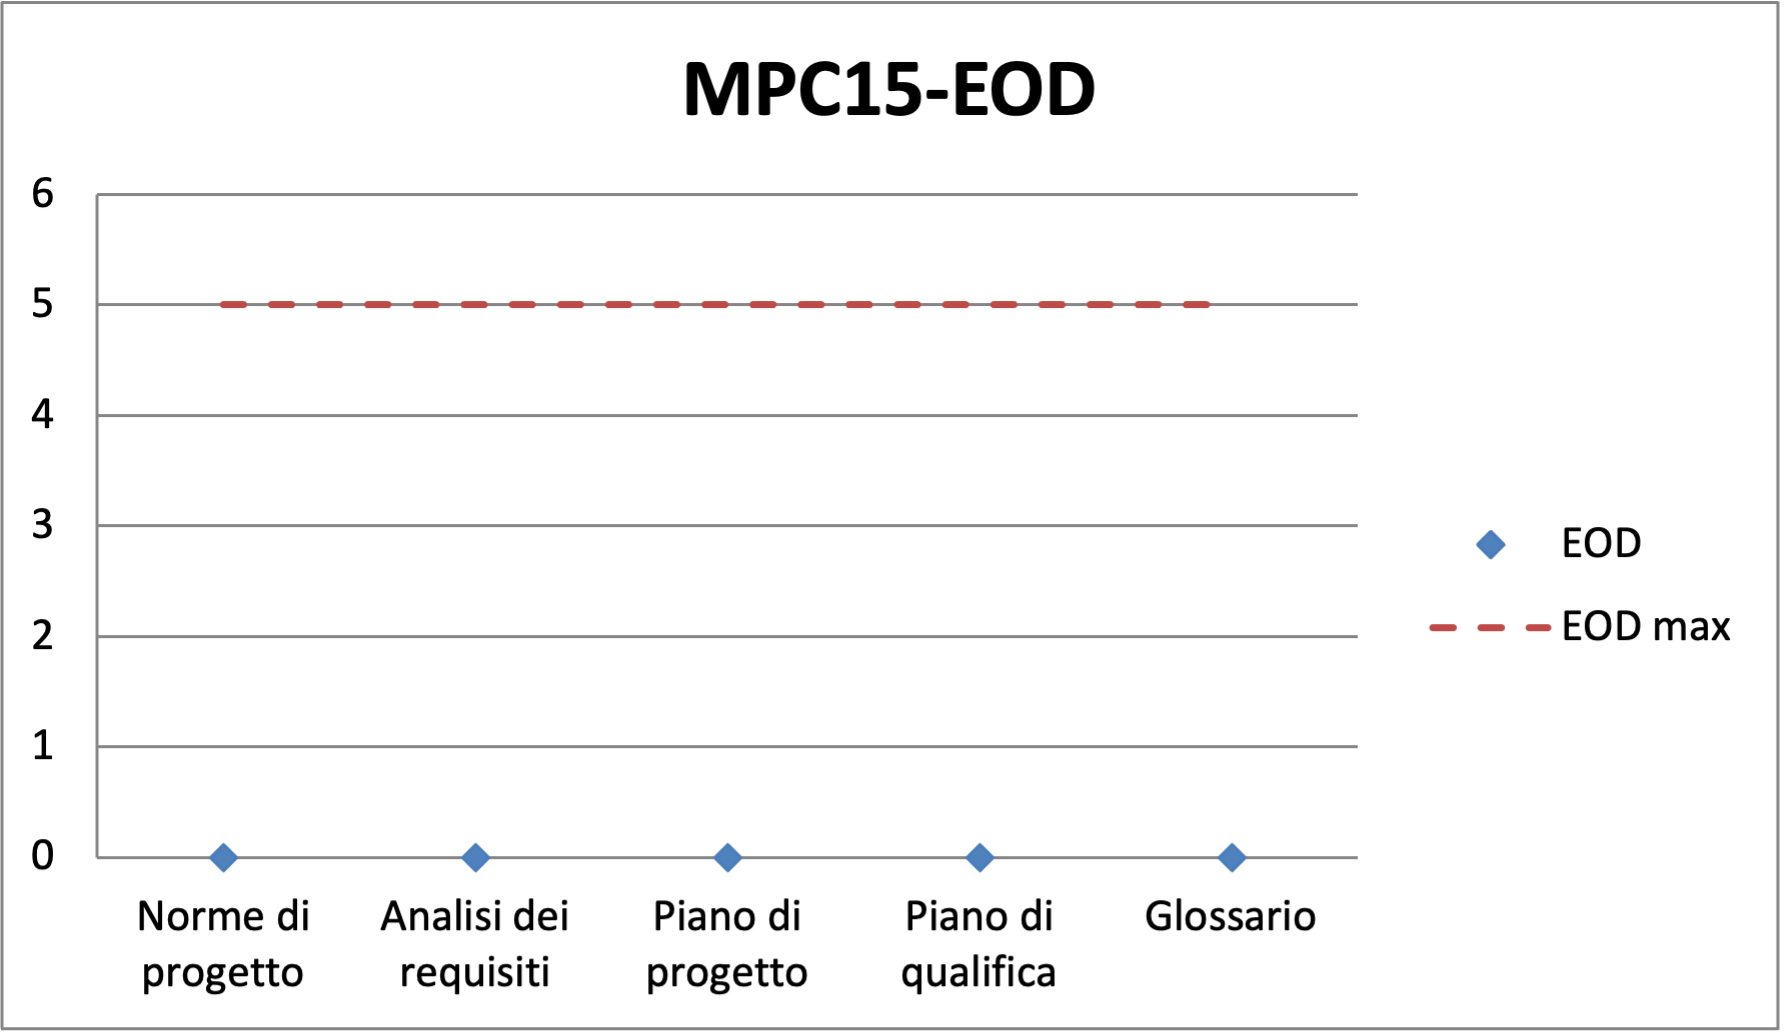
\includegraphics[width=0.8\textwidth]{images/MPC15-EOD.png}
    \caption{MPC15-EOD}
\end{figure}

\newpage

\subsubsection{MPC16-IG}
\begin{figure}[h] 
    \centering
    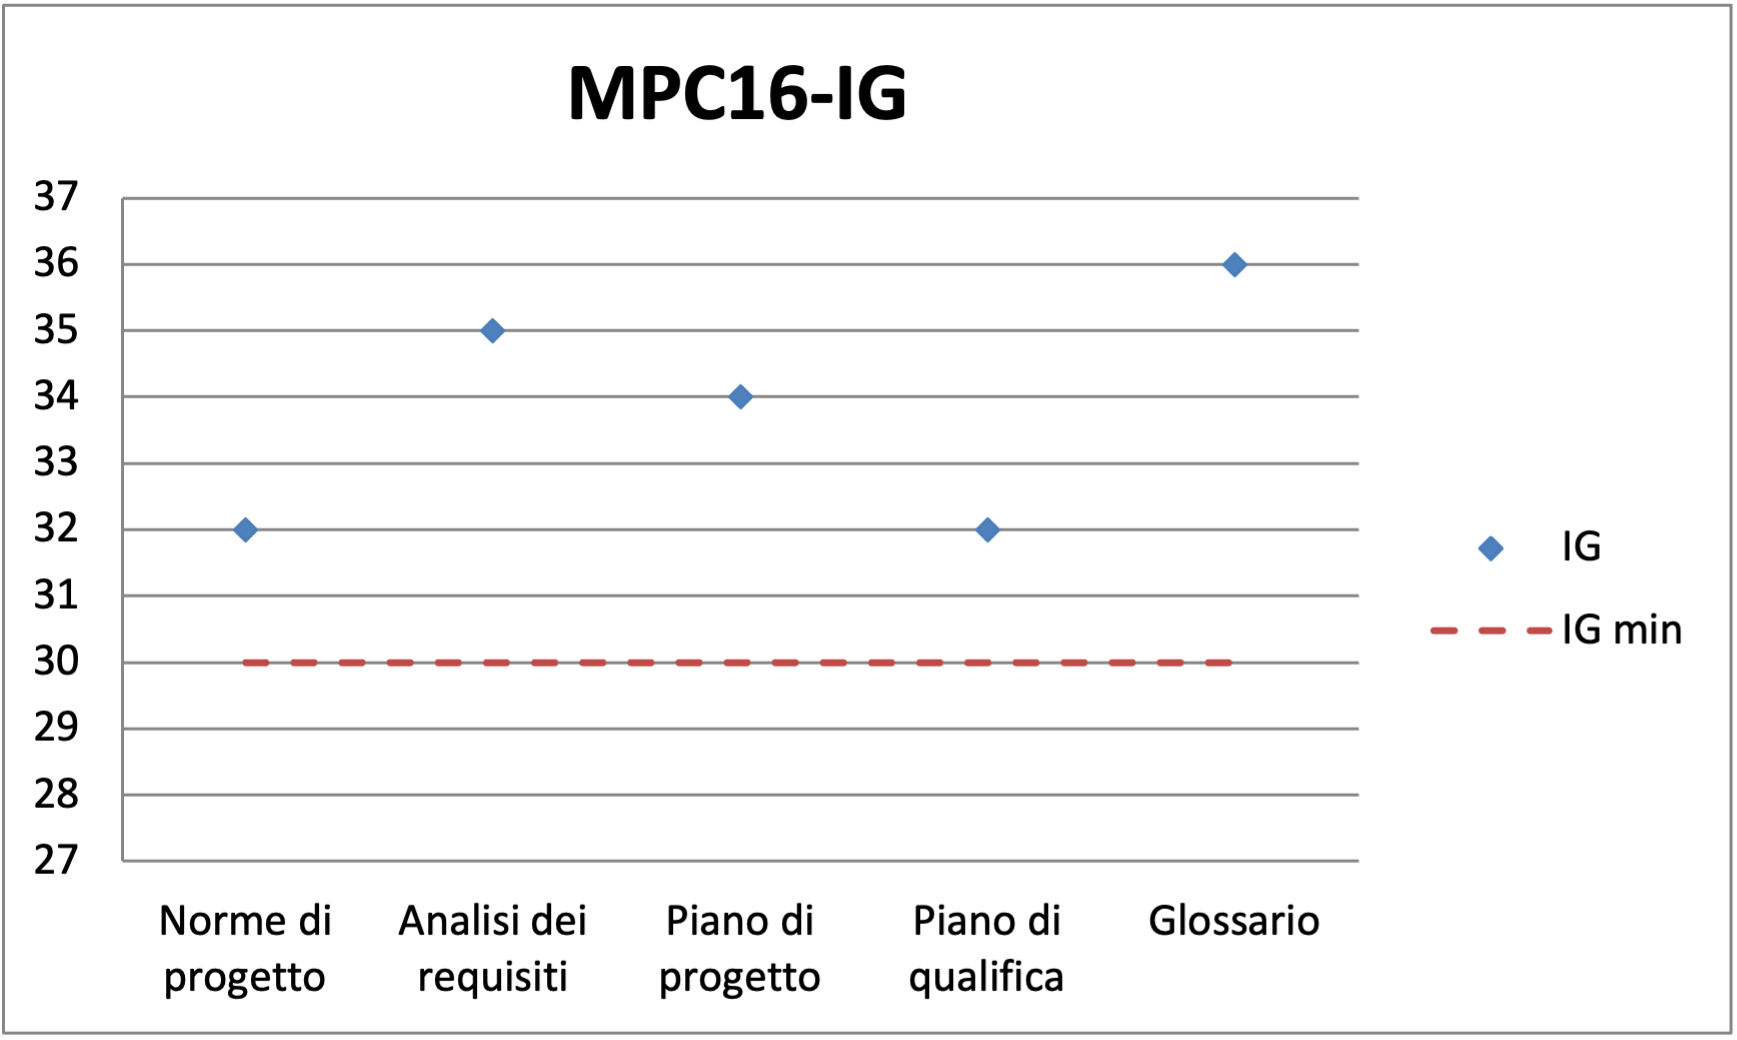
\includegraphics[width=0.8\textwidth]{images/MPC16-IG.png}
    \caption{MPC16-IG}
\end{figure}

\subsubsection{MPC17-MS} \label{sec:accertamento delle qualita}
Le metriche prese in considerazione in questa fase sono:
\begin{itemize}
    \item MPC1-EAC \colorbox{green}{Soddisfatta} 
    \item MPC2-CV \colorbox{green}{Soddisfatta} 
    \item MPC3-SV \colorbox{green}{Soddisfatta}
    \item MPC4-BV \colorbox{green}{Soddisfatta} 
    \item MPC5-PV \colorbox{green}{Soddisfatta} 
    \item MPC6-AC \colorbox{green}{Soddisfatta} 
    \item MPC7-EV \colorbox{green}{Soddisfatta} 
    \item MPC15-EOD \colorbox{green}{Soddisfatta}
    \item MPC16-IG \colorbox{green}{Soddisfatta}
\end{itemize}

La percentuale di metriche soddisfatte (MPC17-MS) equivale al \colorbox{green}{100\%}.

\newpage
\section{Riferimenti esterni} \label{sec:riferimenti_esterni}
Per ulteriori chiarimenti sugli argomenti discussi nel documento, si possono consultare i seguenti link esterni:
\begin{itemize}
    \item Capitolato \textbf{Warehouse Management 3D}:\\
    \url{https://www.math.unipd.it/~tullio/IS-1/2023/Progetto/C5.pdf}
    \item \textbf{Regolamento} del progetto didattico:\\
    \url{https://www.math.unipd.it/~tullio/IS-1/2023/Dispense/PD2.pdf}
    \item Link alla \textbf{documentazione del gruppo}:\\
    \url{https://avant-garde-software-engineering.github.io/documentazione.html}
    \item Standard \textbf{ISO/IEC 12207}, versione 1995:\\
    \url{https://www.math.unipd.it/~tullio/IS-1/2009/Approfondimenti/ISO_12207-1995.pdf}
    \item Metriche di progetto, metodo \textbf{Earned Value}:\\
    \url{https://it.wikipedia.org/wiki/Metriche_di_progetto}
\end{itemize}